\documentclass[12pt]{article}
\usepackage[left=2cm, top=3cm, right=2cm, bottom=3cm]{geometry}
\usepackage[utf8]{inputenc}
\usepackage[T1]{fontenc}
\usepackage[french]{babel}
\usepackage{graphicx}
\usepackage{graphics}
\usepackage{amsmath}
\usepackage{tikz}
\usepackage{graphicx}
\usepackage{xcolor}
\usepackage{parskip}


\title{\textbf{Méthodes expérimentales} \\ TP 3: Chaleur spécifique, calorimétrie}
\author{MENARD Alexandre \\ VIEILLEDENT Florent}

\setlength{\parindent}{1cm}

\begin{document}
\maketitle

\section*{Introduction}
Dans ce travail pratique, on s'intéressera à déterminer les coefficients thermiques, ainsi que les coefficients thermiques
massiques et molaire de l'eau, du vase et de plusieurs métaux. On évaluera également les fuites thermiques du calorimètre pour mettre
en avant de potentielles erreurs dans nos expériences précédentes. \\
On s'appuiera sur des modèles théoriques pour comparer nos mesures à la théorie, et pour effectuer nos comparaisons, on utilisera
les outils numériques adéquats.


\newpage

\section{Première expérience : Détermination de la capacité thermique de l'eau et du vase calorimétrique}

Le but de cette expérience est de déterminer la capacité thermique de l'eau. On va pour cela utiliser principalement un calorimètre et une résistance chauffante de $5 \Omega$, pour pouvoir établir une relation entre la température de l'eau et le temps passé à chauffer de l'eau. On va pouvoir en même temps estimer la capacité thermique du vase calorimétrique. 

\subsection{Expérimentation}

Nous allons effectuer la même expérience pour différentes masses d'eau et pour différents voltages. Pour la première série de mesure, on utilise $450g$ d'eau et une tension de $12V$. On remplit la cuve interne du calorimètre avec la masse d'eau souhaitée, qu'on a pesé avec une balance. On agite l'eau pour que cela soit homogène et on relève la température grâce au thermomètre. On met ensuite en place la résistance chauffante dans l'eau. La résistance est branchée à l'alimentation qui est elle même réglée sur $12V$. On lance le chronomètre et on relève la température toutes les minutes et ceci pendant 15 minutes. On mélange l'eau pendant 15 secondes avant la mesure pour s'assurer que la température soit homogène. 

On recommence ensuite l'expérience avec la même masse d'eau mais une tension de $6V$. Pour la dernière série de mesure, on utilise une tension de $12V$ et une masse d'eau de $800g$.

\subsection{Données}

L'incertitude sur la température nous est donnée par le thermomètre et est de $\pm 0.5^\circ C$, on note donc $\delta T = 0.5^\circ C$. L'incertitude sur la masse est de $\pm 0.1g$ (donnée fourni par la balance). On estime l'incertitude sur le temps à $\pm 1s$, car c'est le temps que nous mettons pour lire le chronomètre puis le thermomètre. L'incertitude sur la tension nous est donnée par la dernière décimale affichée par le générateur, donc $\pm 0.1V$.

	Données pour la première expérience, avec $m_{eau}=450.0\pm 0.1g$ et $U=12.0\pm 0.1V$ :


	Données pour la deuxième expérience, avec $m_{eau}=450.0\pm 0.1g$ et $U=6.0\pm 0.1V$ :
	
	
	Données pour la troisième expérience, avec $m_{eau}=800.0\pm 0.1g$ et $U=12.0\pm 0.1V$ :

\newpage
\subsection{Exploitation des données}

On peut tracer un graphique de la température en fonction du temps.

\begin{figure}[h!]
	\begin{center}
		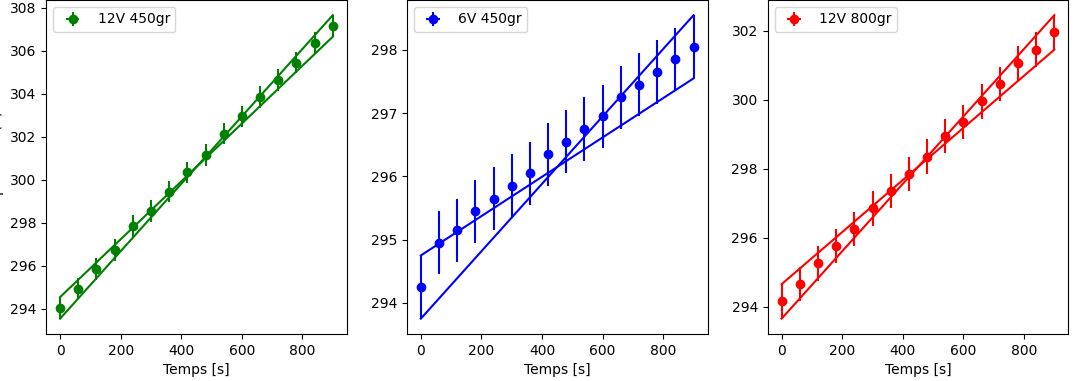
\includegraphics[scale=0.64]{img/Figure_1.png}
	\end{center}
	\label{fig:graph1}
	\caption{Température (en Kelvin) en fonction du temps}
\end{figure}

On trouve une droite dont on peut calculer le coefficient directeur qu'on note a et son incertitude grâce à la méthode des pentes extrêmes.

Soit $t_i, t_f, T_i, T_f$, respectivement le temps initial, final et la température initiale et finale. On applique la formule suivante afin d'obtenir le coefficient directeur $a$ ainsi que l'incertitude associée $\delta a$:

\begin{gather*}
	a_{max} = \frac{(T_f + \delta T) - (T_i - \delta T)}{(t_f - \delta t) - (t_i + dt)} \\
	a_{min} = \frac{(T_f - \delta T) - (T_i + \delta T)}{(t_f + \delta t) - (t_i - dt)} \\
	\\
	a = \frac{a_{max} + a_{min}}{2} \\
	\delta a = \frac{a_{max} - a_{min}}{2}
\end{gather*}

On obtient donc les valeurs suivantes grâce à cette méthode pour les trois expériences:
\begin{itemize}
	\item Expérience 1: $a = 0.015 K.s^{-1}$ et $\delta a = 0.001 K.s^{-1}$
	\item Expérience 2: $a = 0.004 K.s^{-1}$ et $\delta a = 0.001 K.s^{-1}$
	\item Expérience 3: $a = 0.087 K.s^{-1}$ et $\delta a = 0.001 K.s^{-1}$
\end{itemize}

\newpage
Il faut maintenant relier ce coefficient directeur à la capacité thermique $C_V$ du système étudié, ici \{eau+vase calorimétrique\}.
Le système étudié étant un liquide, il a un volume constant et une pression constante et on a :

\begin{equation}
\delta Q=C_VdT
\end{equation}

avec $\delta Q$ la chaleur fourni et $C_V$ la capacité thermique. On suppose ici que $C_V$ est constant sur la gamme de température utilisé, on a donc:

\begin{equation}
Q=C_V\Delta T
\end{equation}

De même on a :

\begin{equation}
Q=P\Delta t
\end{equation}

avec P la puissance fourni et $\Delta t$ la durée pendant laquelle on a injecté du courant dans la résistance. Or $P=UI=\frac{U^2}{R}$ donc:

	\begin{equation}
Q=\frac{U^2}{R}\Delta t = C_V \Delta T 
\Rightarrow \Delta T =\frac{U^2}{RC_V}\Delta t
	\end{equation}

On reconnait ici notre coefficient directeur a, d'où:

\begin{equation}
a=\frac{U^2}{RC_V} \Rightarrow C_V=\frac{U^2}{Ra}
\end{equation}	

Pour calculer notre incertitude on utilise la méthode des dérivés partielles:
\begin{align*}
\Delta C_V &=\displaystyle\left\lvert \frac{\partial C_V}{\partial a}\right\rvert \Delta a + \displaystyle\left\lvert  \frac{\partial C_V}{\partial U}\right\rvert \Delta U \\
&=\frac{U^2}{Ra^2}\Delta a +\frac{2U}{Ra}\Delta U
\end{align*}

Le système étudié est \{eau+vase\}, ainsi, en supposant que les capacités thermiques s'additionnent, on a:
\begin{equation}
C_V=C_{eau}+C_{vase}
\end{equation}

\newpage
On a calculé $C_V$ pour différentes masses d'eau, on peut donc écrire ce système:

\begin{equation}
	\begin{split}
		\begin{cases}
			C_{V1}=C_{eau1}+C_{vase} \\
			C_{V3}=C_{eau3}+C_{vase}
		\end{cases} 
&\Rightarrow 
		\begin{cases}
			C_{vase}=C_{V1}-c_{eau}m_{eau1} \\
			c_{eau}m_{eau3}=C_{V3}-C_{vase}
		\end{cases} \\
&\Rightarrow 
		\begin{cases}
			C_{vase}=C_{V1}-\frac{(C_{V3}-C_{Vase})}{m_{eau3}} \\
			c_{eau}=\frac{C_{V3}-C_{vase}}{m_{eau3}}
		\end{cases} \\
&\Rightarrow 
		\begin{cases}
			C_{vase}(m_{eau3}-m_{eau1})=C_{V1}m_{eau3}-C_{V3}m_{eau1} \\
			c_{eau}=\frac{C_{V3}-C_{vase}}{m_{eau3}}
		\end{cases} \\
&\Rightarrow 		
		\begin{cases}
			C_{vase}=\frac{C_{V1}m_{eau3}-C_{V3}m_{eau1}}{m_{eau3}-m_{eau1}}  \\
			c_{eau}=\frac{C_{V3}-C_{vase}}{m_{eau3}}
		\end{cases}
	\end{split}	
\end{equation}
Calculs des incertitudes:

\begin{align*}
\Delta C_{vase} &= \displaystyle\left\lvert \frac{\partial C_{vase}}{\partial C_{V1}}\right\rvert \Delta C_{V1}+ \displaystyle\left\lvert \frac{\partial C_{vase}}{\partial C_{V3}}\right\rvert \Delta C_{V3} +\displaystyle\left\lvert \frac{\partial C_{vase}}{\partial m_{eau3}}\right\rvert \Delta m_{eau3} + \displaystyle\left\lvert \frac{\partial C_{vase}}{\partial m_{eau1}}\right\rvert \Delta m_{eau1} \\
&= \frac{\displaystyle\left\lvert m_{eau3}-C_{V3}m_{eau1}\right\rvert \Delta C_{V1} + \displaystyle\left\lvert m_{eau3}C_{V1}-m_{eau1}\right\rvert \Delta C_{V3}}{m_{eau3}-m_{eau1}}\\
&+ \frac{\displaystyle\left\lvert m_{eau1}(C_{V3}-C_{V1})\right\rvert \Delta m_{eau1}+\displaystyle\left\lvert m_{eau1}(2C_{V3}-C_{V1})-m_{eau3}(C_{V3}+C_{V1})\right\rvert \Delta m_{eau3} }{(m_{eau3}-m_{eau1})^2} \\
&=
\end{align*}

\begin{align*}
\Delta c_{eau} &= \displaystyle\left\lvert \frac{\partial c_{eau}}{\partial C_{V}}\right\rvert \Delta C_{V} + \displaystyle\left\lvert \frac{\partial c_{eau}}{\partial C_{vase}}\right\rvert \Delta C_{vase} + \displaystyle\left\lvert  \frac{\partial c_{Veau}}{\partial m_{eau}}\right\rvert \Delta m_{eau} \\
	&=	\frac{C_{vase}}{m_{eau}}\Delta C_{V} + \frac{C_{V}}{m_{eau}}\Delta C_{vase} + \frac{C_{V}-C_{vase}}{m_{eau}^2}\Delta m_{eau}
\end{align*}


\subsection{Interprétation}

La valeur théorique de la capacité thermique massique de l'eau est $c_{vth }=4185 ~ J.kg^{-1}.K^{-1}$

\newpage
\section{Deuxième expérience : Capacités thermiques massiques de quelque solides}

Le but de cette expérience est de déterminer la capacité massique du duralumin, du laiton, du téflon et du plexiglas. On utilisera pour cela la relation suivante:

\begin{equation}
	T_f=\frac{C_0T_0+C_1T_1}{C_0+C_1}
\label{EquationTf}
\end{equation}
avec $C_0$ la capacité thermique du système \{eau+vase\}, $C_1$ la capacité thermique du métal, $T_0$ la température initial de l'eau, $T_1$ la température initial du métal et $T_F$ la température final de l'eau.

\subsection{Expérimentation}
On place $450g$ d'eau dans le calorimètre et on mesure sa température après avoir agité. On place un morceau du solide qu'on souhaite étudié dans de l'eau bouillante, dont on mesure aussi la température. Après quelques minutes, on retire le solide de l'eau bouillante et on le met dans le calorimètre. On agite en continue l'eau tout en surveillant la température. On note cette dernière lorsqu'elle atteint un maximum. On retire ensuite le solide et on le pèse après l'avoir séché.

\subsection{Données}
On reprend les notations de l'équation (\ref{EquationTf}). Les incertitudes sont données par la balance et le thermomètre. Pour tous les solides, on a $T_1=94.6\pm 0.5^{\circ}C$
\begin{table}[h!]
	\begin{center}
		\begin{tabular}{|c|c|c|c|c|}
		\hline
		Solide & $m_{eau} \pm 0.1g$ & $m_{solide}\pm 0.1g$ & $T_0\pm 0.5^{\circ}C$ & $T_f\pm 0.5^{\circ}C$\\ \hline
		Laiton & $451.1$ & $82.7$ & $21.1$ & $22.4$ \\
		Téflon & $451.1$ & $32.5$ & $22.3$ & $23.4$ \\
		Plexiglas & $450.0$ & $47.8$ & $22.3$ & $23.4$ \\
		Duralumin & $452.5$ & $77.2$ & $21.1$ & $24.0$ \\ \hline
		\end{tabular}
		\caption{Mesures pour les différents solides de l'expérience 2}
		\label{table:mesureexp2}
	\end{center}
\end{table}

\subsection{Exploitation des données}
On calcule d'abord la capacité thermique $C_0$ du système \{eau+vase\}:
\begin{equation}
C_0=c_{eau}m_{eau}+C_{vase}
\end{equation}
On utilise la capacité thermique massique théorique de l'eau et la capacité du vase que nous avons calculé précédemment. Calcul des incertitudes
\begin{align*}
\Delta C_0&=\displaystyle\left\lvert \frac{\partial C_0}{\partial m_{eau}}\right\rvert \Delta m_{eau} + \displaystyle\left\lvert \frac{\partial C_0}{\partial C_{vase}}\right\rvert \Delta C_{vase}\\
&=c_{eau}\Delta m_{eau}+\Delta C_{vase}
\end{align*}



On cherche la capacité thermique molaire des matériaux. On va déterminé la capacité thermique du solide grâce à l'équation (\ref{EquationTf}):
\begin{align*}
T_f=\frac{C_0T_0+C_1T_1}{C_0+C_1} &\Rightarrow T_FC_0+T_FC_1=C_OT_0+C_1T_1 \\
&\Rightarrow C_1(T_F-T_1)=C_0(T_0-T_F) \\
&\Rightarrow C_1=\frac{C_0(T_0-T_F)}{T_F-T_1}
\end{align*}

On calcule l'incertitude associée:
\begin{align*}
\Delta C_1 &= \displaystyle\left\lvert \frac{\partial C_1}{\partial C_0}\right\rvert \Delta C_0 + \displaystyle\left\lvert \frac{\partial C_1}{\partial T_0}\right\rvert \Delta T_0 + \displaystyle\left\lvert \frac{\partial C_1}{\partial T_1}\right\rvert \Delta T_1 + \displaystyle\left\lvert \frac{\partial C_1}{\partial T_F}\right\rvert \Delta T_F \\
&= \frac{T_0-T_F}{T_F-T_1}\Delta C_0 + \frac{C_0T_F}{T_1-T_F}\Delta T_0 + \frac{\displaystyle\left\lvert C_0T_F(T_0-T_F)  \right\rvert}{(T_F-T_1)^2}\Delta T_1 + \frac{\displaystyle\left\lvert C_0((T_F-T_1)-T_1(T_0-T_F))   \right\rvert}{(T_F-T_1)^2}\Delta T_F
\end{align*}




On peut maintenant calculer la capacité thermique massique pour chaque solide:
\begin{equation}
c_{solide}=\frac{C_1}{m_{solide}}
\end{equation}
Il faut maintenant calculer la masse molaire de chaque matériaux. On a déjà la formule brute du plexiglas ($C_5H_8O_2$) et du téflon ($C_2F_4$). On peut donc facilement calculer leur masse molaire:
\begin{align*}
M_{plexiglas}&=5M_C+8M_H+2M_O & M_{teflon}&=2M_C+4M_F  \\
&=5\times 12+8+2\times 16 & &=2\times 12+4\times 19 \\
&=100\, g.mol^{-1} & &=100\, g.mol^{-1}
\end{align*}

Pour le laiton et le duralumin, il faut calculer la masse molaire du matériaux à partir des proportions massique qu'on note $w_{i}$. 

On fait l'application numérique pour le laiton et le duralumin,avec:

	-les fraction massiques pour le laiton: $w_{zinc}=0.4$, $w_{plomb}=0.02$, $w_{cuivre}=0.58$
	
	-les fractions massiques pour le duralumin: $w_{silicium}=0.005$, $w_{fer}=0.0035$, $w_{cuivre}=0.04$, $w_{manganese}=0.007$, $w_{magnesium}=0.007$, $w_{zinc}=0.0025$, $w_{aluminium}=0.935$
	
	


On utilise maintenant la relation : $c_{molaire}=c_{solide}M_{solide}$ et on regroupe nos résultats dans un tableau.
\begin{table}[h!]
	\begin{center}
		\begin{tabular}{|c|c|c|c|c|c|}
		\hline
		Solide & $C_0(J.K^{-1})$ & $C_1(J.K^{-1})$ & $c_{solide}(J.kg^{-1}.K^{-1})$ & $M_{solide}(g.mol^{-1})$ & $c_{molaire}(J.mol^{-1}.K^{-1})$ \\
		\hline

	
		\end{tabular}
	\end{center}		
\end{table}


\end{document}
